\documentclass{article}
\usepackage{graphicx}   % Importing graphics
\usepackage{graphics}   % Importing graphics
\usepackage{hyperref}   % Hyperlink references and URLs
\title{Prototype Review Document}
\author{
	Frank Clark \\\url{francis.j.clark@drexel.edu}
    \and Dustin Ingram \\\url{dustin.s.ingram@drexel.edu}
	\and Maria Kolakowska \\\url{maria.j.kolakowska@drexel.edu}
    \and Aaron Rosenfeld \\\url{aaron.rosenfeld@drexel.edu}
}
\begin{document}

\maketitle

\section{Introduction}
The prototye represents the integration of a simulator with basic functionality as well as a Display Tool (SDT). The prototype fulfills a number of goals, as well as frames the work needed to be done in the next version.
\subsection{Prototype Goals Completed}
\begin{itemized}
    \item Created a simulator which aggregates a user-defined Scenario and Network.
    \item Specified a rough format for the user-definition of Scenarios, Networks and Agents.
    \item Implemented a Display Tool based on a real-world model which displays, verbatim, the real-time events created by the simulator.
    \item Allowed agents to react in real-time to events distributed through the simulator by other agents.
    \item Created a simplified process for using an Agent to publish real-world data into the simulator.
    \item Created an API channel for the simulator which allows the subscription and publication of events.
\end{itemized}
\section{Sample Configuration Files}
The following files represent the sample configuration files for the Scenario Definition and the Network Topology Definition, which are interpreted by the simulator to set up the virtual nodes, their agents, and settings.
\subsection{Scenario}
This sample Scenario Configuration defines a scenario with 5 nodes, each with a local `Moving' agent which has been independently defined to take a random walk within the limits of the scenario. The configuration makes the node model, applies the user-defined agent, and adds the node to the Scenario. 

\begin{verbatim}
from stage.scenario import Scenario
from stage.model import Model
from stage.agents.testagent import TestAgent
from stage.agents.randommoveagent import MovingAgent
from stage.agents.circlewalker import CircleWalkerAgent

class ScenarioDef(Scenario) :
    def __init__(self) :
        Scenario.__init__(self)

        for node_id in range(0, 5) :
            node = Model(name='n%s' % node_id, position=(0,0,0), \
                agents = [], interfaces = {})
            agent_instance = MovingAgent()
            node.get('agents').append(agent_instance)
            self._nodes.append(node)
\end{verbatim}

\subsection{Network}
This sample Network Configuration sets one wireles interface for each node in the scenario.
\begin{verbatim}
from stage.network import Network
from stage.model import Model

class NetworkConcrete(Network) :
    def __init__(self, scen_inst) :
        Network.__init__(self, scen_inst)

        for node in self._scen_inst.get_nodes() :
            node.get('interfaces')['eth0'] = Model(type='wireless', \
                range=20, ssid='wlan0')
\end{verbatim}

\section{Screenschots of SDT-3D (STAGE Display Tool)}
The nodes in their initial state:
\center{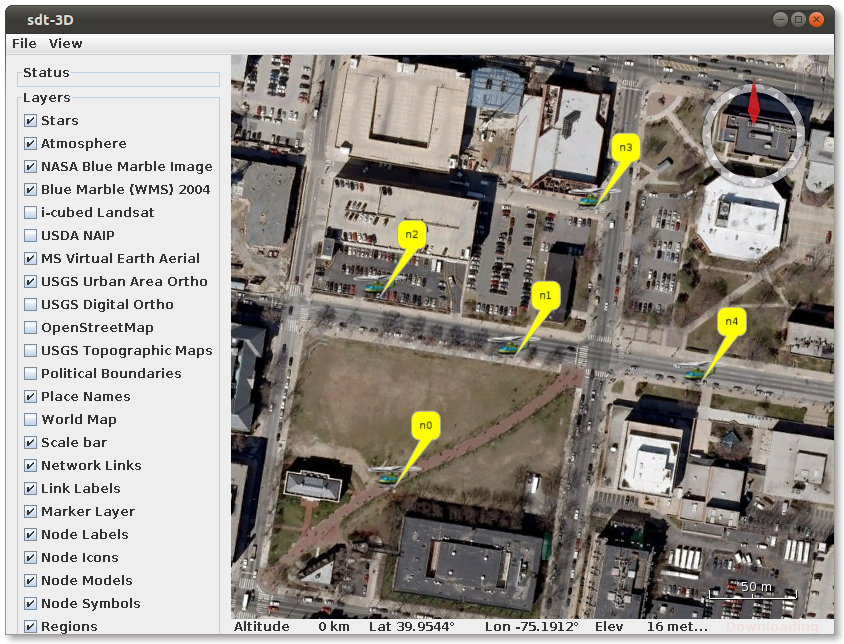
\includegraphics[scale=.3]{images/ss1.png}}

After a few ticks, some nodes have become linked and can communicate:
\center{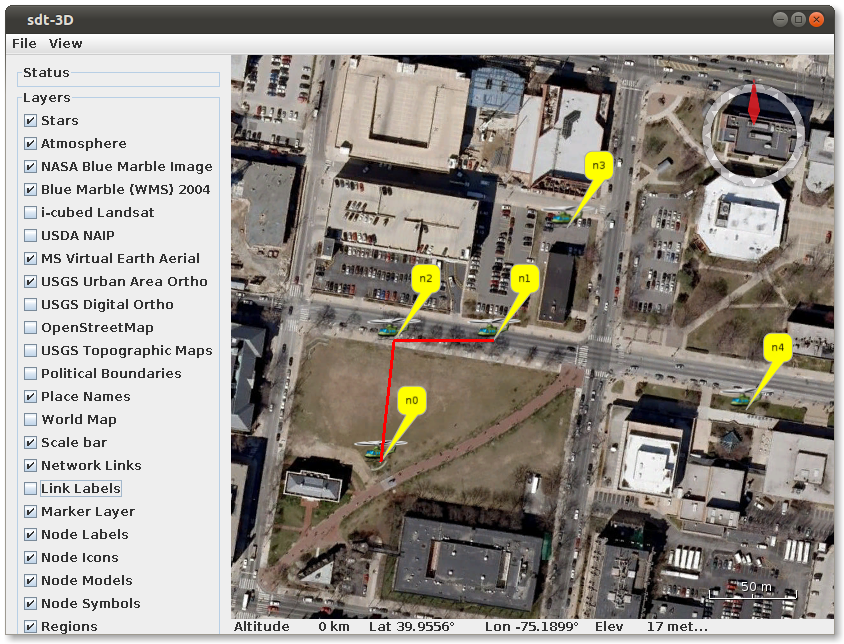
\includegraphics[scale=.3]{images/ss2.png}}

All nodes are now connected to form a static network:
\center{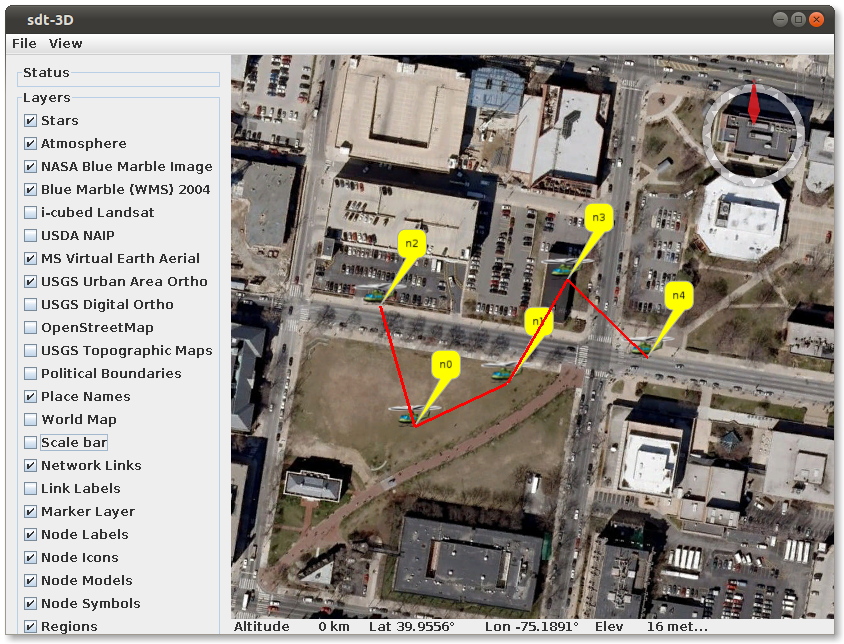
\includegraphics[scale=.3]{images/ss3.png}}

\end{document}
